%==============================================================================
% UniVR Chatbot - Project Documentation
% A RAG-Powered AI Assistant for University of Verona
%==============================================================================

\documentclass[12pt,a4paper]{article}

%------------------------------------------------------------------------------
% Packages
%------------------------------------------------------------------------------
\usepackage[utf8]{inputenc}
\usepackage[T1]{fontenc}
\usepackage{graphicx}
\usepackage{geometry}
\usepackage{hyperref}
\usepackage{xcolor}
\usepackage{tikz}
\usepackage{tcolorbox}
\usepackage{enumitem}
\usepackage{booktabs}
\usepackage{fancyhdr}
\usepackage{titlesec}
\usepackage{float}

% TikZ libraries
\usetikzlibrary{shapes.geometric, arrows.meta, positioning, fit, backgrounds, calc}

%------------------------------------------------------------------------------
% Page Setup
%------------------------------------------------------------------------------
\geometry{
    left=2.5cm,
    right=2.5cm,
    top=3cm,
    bottom=3cm
}

% Colors
\definecolor{univrred}{RGB}{187, 0, 0}
\definecolor{univrbg}{RGB}{245, 245, 250}
\definecolor{darkblue}{RGB}{30, 60, 120}
\definecolor{lightblue}{RGB}{200, 220, 255}

% Header/Footer
\pagestyle{fancy}
\fancyhf{}
\fancyhead[L]{\footnotesize UniVR Chatbot Documentation}
\fancyhead[R]{\footnotesize \thepage}
\renewcommand{\headrulewidth}{0.4pt}

% Section formatting
\titleformat{\section}
    {\Large\bfseries\color{univrred}}
    {\thesection}{1em}{}[\titlerule]
\titleformat{\subsection}
    {\large\bfseries\color{darkblue}}
    {\thesubsection}{1em}{}

% Hyperref setup
\hypersetup{
    colorlinks=true,
    linkcolor=darkblue,
    urlcolor=univrred,
    citecolor=darkblue
}

%------------------------------------------------------------------------------
% TikZ Styles
%------------------------------------------------------------------------------
\tikzstyle{component} = [
    rectangle, 
    rounded corners=8pt, 
    minimum width=3cm, 
    minimum height=1.2cm, 
    text centered, 
    draw=darkblue, 
    fill=lightblue,
    font=\small\bfseries
]
\tikzstyle{database} = [
    cylinder, 
    shape border rotate=90, 
    aspect=0.25, 
    minimum width=2.5cm, 
    minimum height=1.5cm, 
    draw=darkblue, 
    fill=lightblue!60
]
\tikzstyle{user} = [
    circle, 
    minimum size=1.2cm, 
    draw=univrred, 
    fill=univrred!15,
    font=\small\bfseries
]
\tikzstyle{arrow} = [
    thick, 
    ->, 
    >=Stealth, 
    color=darkblue
]
\tikzstyle{dashedarrow} = [
    thick, 
    dashed, 
    ->, 
    >=Stealth, 
    color=gray
]

%==============================================================================
% Document Begin
%==============================================================================
\begin{document}

%------------------------------------------------------------------------------
% Title Page
%------------------------------------------------------------------------------
\begin{titlepage}
    \centering
    \vspace*{2cm}
    
    {\Huge\bfseries\color{univrred} UniVR Chatbot\par}
    \vspace{0.5cm}
    {\Large A RAG-Powered AI Assistant\par}
    {\Large for the University of Verona\par}
    
    \vspace{2cm}
    
    % Simple illustration
    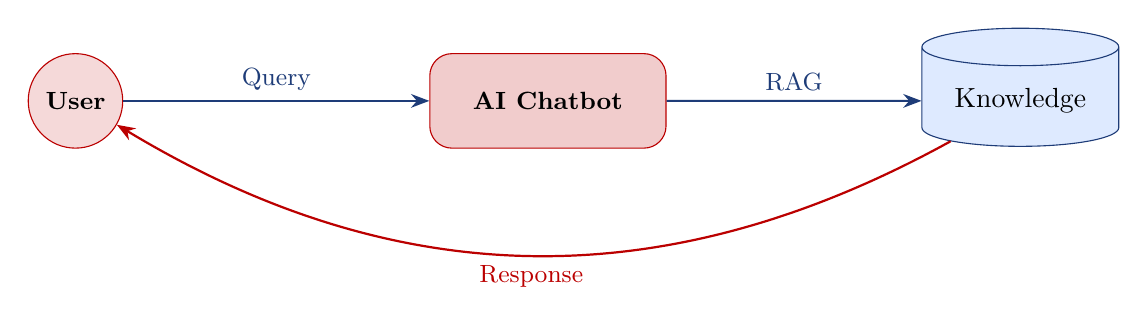
\begin{tikzpicture}[scale=1.2]
        % User icon
        \node[user] (user) at (0,0) {User};
        
        % Chatbot icon
        \node[component, fill=univrred!20, draw=univrred] (bot) at (5,0) {AI Chatbot};
        
        % Knowledge base
        \node[database] (kb) at (10,0) {Knowledge};
        
        % Arrows
        \draw[arrow] (user) -- node[above]{\small Query} (bot);
        \draw[arrow] (bot) -- node[above]{\small RAG} (kb);
        \draw[arrow, color=univrred] (kb) to[bend left=30] node[below]{\small Response} (user);
    \end{tikzpicture}
    
    \vspace{3cm}
    
    {\large\textbf{Project Documentation}\par}
    \vspace{0.5cm}
    {\large Version 1.0\par}
    
    \vfill
    
    {\normalsize Università degli Studi di Verona\par}
    {\normalsize \today\par}
\end{titlepage}

%------------------------------------------------------------------------------
% Table of Contents
%------------------------------------------------------------------------------
\tableofcontents
\newpage

%==============================================================================
% Section 1: Introduction
%==============================================================================
\section{Introduction}

\subsection{Project Overview}

The \textbf{UniVR Chatbot} is an AI-powered conversational assistant designed to help students at the University of Verona find accurate and relevant information about university services. The chatbot leverages \textbf{Retrieval-Augmented Generation (RAG)} to provide responses grounded in official university documents.

\begin{tcolorbox}[colback=univrbg, colframe=univrred, title=\textbf{Key Features}]
    \begin{itemize}[noitemsep]
        \item \textbf{Intelligent Q\&A}: Natural language understanding for student queries
        \item \textbf{Document-Grounded Responses}: Answers based on official university documents
        \item \textbf{Multi-Domain Support}: Specialized knowledge bases for different topics
        \item \textbf{Bilingual Support}: Italian and English language capabilities
        \item \textbf{Source Citations}: Transparent references to source documents
    \end{itemize}
\end{tcolorbox}

\subsection{Problem Statement}

Students often struggle to find specific information about:
\begin{itemize}
    \item Scholarship opportunities and application deadlines
    \item Tuition fees and payment schedules
    \item Admission requirements for various programs
    \item International student services and visa procedures
\end{itemize}

The traditional approach of navigating through multiple web pages and PDF documents is time-consuming and often leads to missed deadlines or incomplete information.

\subsection{Solution}

The UniVR Chatbot addresses these challenges by:
\begin{enumerate}
    \item \textbf{Centralizing Information}: All relevant documents are indexed in searchable knowledge bases
    \item \textbf{Providing Instant Answers}: Students get immediate responses to their questions
    \item \textbf{Ensuring Accuracy}: Responses are grounded in official documents, reducing misinformation
    \item \textbf{Offering Guidance}: The chatbot suggests relevant questions to help students discover information
\end{enumerate}

%==============================================================================
% Section 2: System Architecture
%==============================================================================
\section{System Architecture}

\subsection{High-Level Architecture}

The UniVR Chatbot follows a modern three-tier architecture with a clear separation between the frontend, backend, and AI services.

\begin{figure}[H]
    \centering
    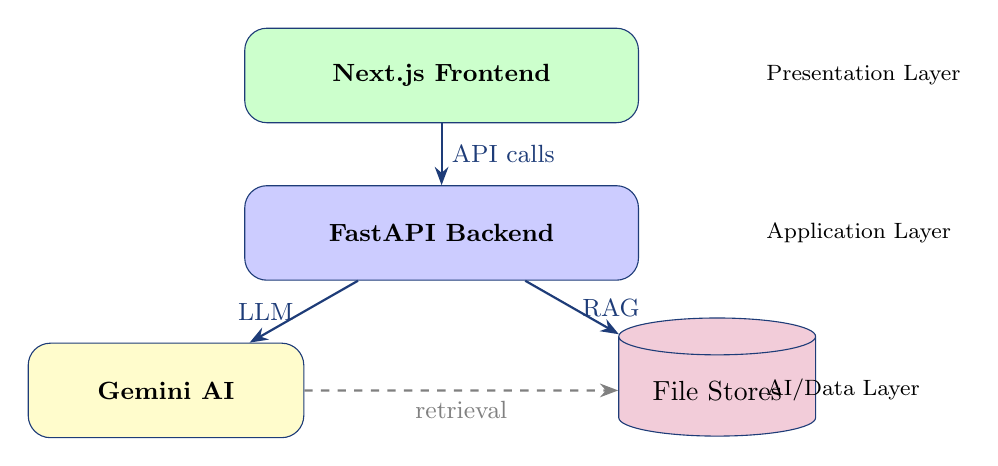
\begin{tikzpicture}[node distance=2cm]
        % Frontend Layer
        \node[component, fill=green!20, minimum width=5cm] (frontend) at (0, 4) {Next.js Frontend};
        
        % Backend Layer
        \node[component, fill=blue!20, minimum width=5cm] (backend) at (0, 2) {FastAPI Backend};
        
        % AI Layer
        \node[component, fill=yellow!20, minimum width=3.5cm] (gemini) at (-3.5, 0) {Gemini AI};
        \node[database, fill=purple!20] (stores) at (3.5, 0) {File Stores};
        
        % Connections
        \draw[arrow] (frontend) -- node[right]{\small API calls} (backend);
        \draw[arrow] (backend) -- node[left]{\small LLM} (gemini);
        \draw[arrow] (backend) -- node[right]{\small RAG} (stores);
        \draw[dashedarrow] (gemini) -- node[below]{\small retrieval} (stores);
        
        % Labels
        \node[anchor=west] at (4, 4) {\footnotesize Presentation Layer};
        \node[anchor=west] at (4, 2) {\footnotesize Application Layer};
        \node[anchor=west] at (4, 0) {\footnotesize AI/Data Layer};
    \end{tikzpicture}
    \caption{Three-tier architecture of the UniVR Chatbot}
    \label{fig:architecture}
\end{figure}

\subsection{Component Description}

\begin{table}[H]
    \centering
    \begin{tabular}{@{}llp{7cm}@{}}
        \toprule
        \textbf{Layer} & \textbf{Technology} & \textbf{Responsibility} \\
        \midrule
        Frontend & Next.js & User interface, domain selection, chat display \\
        Backend & FastAPI & API endpoints, request routing, agent orchestration \\
        AI Service & Gemini & Natural language processing, response generation \\
        Knowledge & File Stores & Document indexing, semantic search, RAG retrieval \\
        \bottomrule
    \end{tabular}
    \caption{Component technologies and responsibilities}
\end{table}

%==============================================================================
% Section 3: RAG Concept
%==============================================================================
\section{Understanding RAG (Retrieval-Augmented Generation)}

\subsection{What is RAG?}

\textbf{Retrieval-Augmented Generation (RAG)} is a technique that enhances AI responses by combining:
\begin{enumerate}
    \item \textbf{Retrieval}: Finding relevant documents from a knowledge base
    \item \textbf{Generation}: Creating natural language responses using an LLM
\end{enumerate}

\begin{figure}[H]
    \centering
    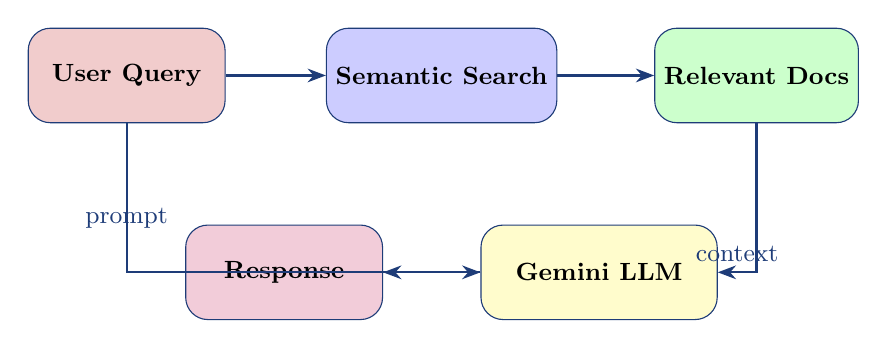
\begin{tikzpicture}[node distance=1.5cm]
        % User Query
        \node[component, fill=univrred!20, minimum width=2.5cm] (query) at (0, 0) {User Query};
        
        % Retrieval
        \node[component, fill=blue!20, minimum width=2.5cm] (search) at (4, 0) {Semantic Search};
        
        % Documents
        \node[component, fill=green!20, minimum width=2.5cm] (docs) at (8, 0) {Relevant Docs};
        
        % LLM
        \node[component, fill=yellow!20, minimum width=3cm] (llm) at (6, -2.5) {Gemini LLM};
        
        % Response
        \node[component, fill=purple!20, minimum width=2.5cm] (response) at (2, -2.5) {Response};
        
        % Arrows
        \draw[arrow] (query) -- (search);
        \draw[arrow] (search) -- (docs);
        \draw[arrow] (docs) |- node[near end, above]{\small context} (llm);
        \draw[arrow] (query) |- node[near start, below]{\small prompt} (llm);
        \draw[arrow] (llm) -- (response);
    \end{tikzpicture}
    \caption{RAG workflow: retrieval enhances generation with relevant context}
    \label{fig:rag}
\end{figure}

\subsection{Benefits of RAG}

\begin{tcolorbox}[colback=univrbg, colframe=darkblue]
    \begin{description}[style=nextline]
        \item[Accuracy] Responses are grounded in actual documents, reducing hallucinations
        \item[Up-to-date Information] New documents can be added without retraining the model
        \item[Transparency] Sources can be cited, allowing users to verify information
        \item[Domain Specificity] Knowledge bases can be tailored to specific topics
    \end{description}
\end{tcolorbox}

\subsection{Multi-Domain RAG Architecture}

The UniVR Chatbot implements a \textbf{multi-domain RAG architecture}, where each knowledge domain (scholarships, admissions, etc.) has its own dedicated File Search Store.

\begin{figure}[H]
    \centering
    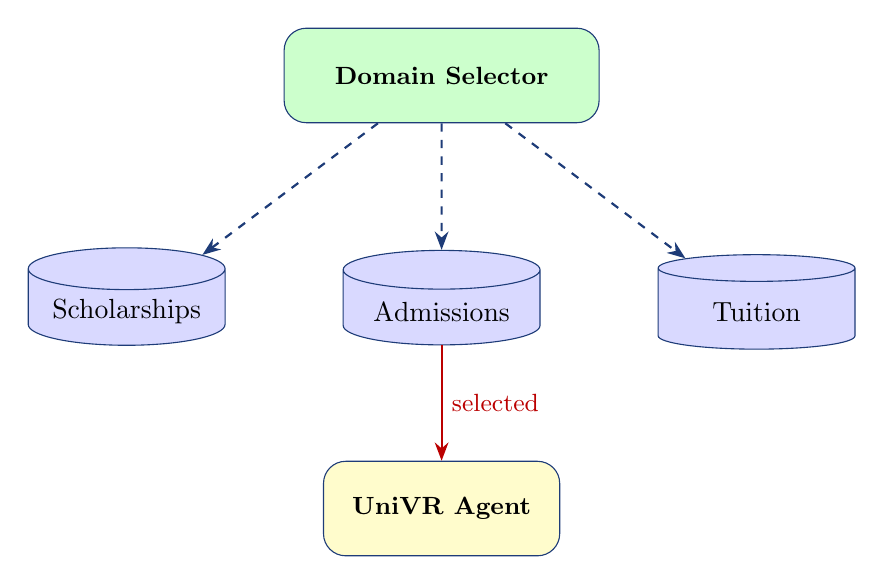
\begin{tikzpicture}[node distance=1.2cm]
        % Domain Selector
        \node[component, fill=green!20, minimum width=4cm] (selector) at (0, 3) {Domain Selector};
        
        % Domains
        \node[database, fill=blue!15, minimum height=1.2cm] (d1) at (-4, 0) {Scholarships};
        \node[database, fill=blue!15, minimum height=1.2cm] (d2) at (0, 0) {Admissions};
        \node[database, fill=blue!15, minimum height=1.2cm] (d3) at (4, 0) {Tuition};
        
        % Agent
        \node[component, fill=yellow!20, minimum width=3cm] (agent) at (0, -2.5) {UniVR Agent};
        
        % Arrows from selector
        \draw[arrow, dashed] (selector) -- (d1);
        \draw[arrow, dashed] (selector) -- (d2);
        \draw[arrow, dashed] (selector) -- (d3);
        
        % Arrow to agent (selected domain)
        \draw[arrow, thick, color=univrred] (d2) -- node[right]{\small selected} (agent);
    \end{tikzpicture}
    \caption{Multi-domain architecture: user selects a domain, agent uses corresponding knowledge base}
    \label{fig:multidomain}
\end{figure}

%==============================================================================
% Section 4: Data Flow
%==============================================================================
\section{Data Flow}

\subsection{Complete Request-Response Cycle}

The following diagram illustrates the complete data flow from user query to response display.

\begin{figure}[H]
    \centering
    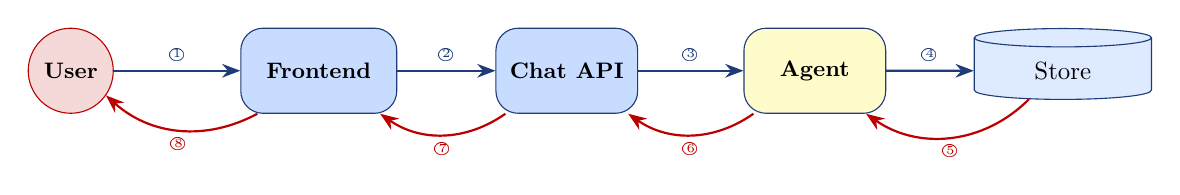
\begin{tikzpicture}[node distance=1cm, scale=0.9, transform shape]
        % Nodes
        \node[user] (user) at (0, 0) {User};
        \node[component, minimum width=2.2cm] (fe) at (3.5, 0) {Frontend};
        \node[component, minimum width=2cm] (api) at (7, 0) {Chat API};
        \node[component, minimum width=2cm, fill=yellow!20] (agent) at (10.5, 0) {Agent};
        \node[database, minimum height=1cm] (store) at (14, 0) {Store};
        
        % Flow arrows - top (request)
        \draw[arrow] (user) -- node[above, font=\tiny]{\textcircled{1}} (fe);
        \draw[arrow] (fe) -- node[above, font=\tiny]{\textcircled{2}} (api);
        \draw[arrow] (api) -- node[above, font=\tiny]{\textcircled{3}} (agent);
        \draw[arrow] (agent) -- node[above, font=\tiny]{\textcircled{4}} (store);
        
        % Flow arrows - bottom (response)
        \draw[arrow, color=univrred] (store) to[bend left=40] node[below, font=\tiny]{\textcircled{5}} (agent);
        \draw[arrow, color=univrred] (agent) to[bend left=35] node[below, font=\tiny]{\textcircled{6}} (api);
        \draw[arrow, color=univrred] (api) to[bend left=35] node[below, font=\tiny]{\textcircled{7}} (fe);
        \draw[arrow, color=univrred] (fe) to[bend left=35] node[below, font=\tiny]{\textcircled{8}} (user);
    \end{tikzpicture}
    \caption{Request-response data flow}
    \label{fig:dataflow}
\end{figure}

\subsection{Step-by-Step Process}

\begin{enumerate}
    \item \textbf{User Input}: User types a question in the chat interface
    \item \textbf{API Request}: Frontend sends message + selected domain to backend
    \item \textbf{Agent Invocation}: Chat API initializes the UniVR Agent with domain context
    \item \textbf{Document Retrieval}: Agent uses File Search to find relevant documents
    \item \textbf{Context Injection}: Retrieved documents are provided as context to Gemini
    \item \textbf{Response Generation}: Gemini generates a grounded response
    \item \textbf{API Response}: Backend returns response with source citations
    \item \textbf{Display}: Frontend renders the formatted response with sources
\end{enumerate}

%==============================================================================
% Section 5: Frontend User Flow
%==============================================================================
\section{Frontend User Flow}

\subsection{User Journey Overview}

The frontend provides an intuitive flow that guides users from domain selection to conversation.

\begin{figure}[H]
    \centering
    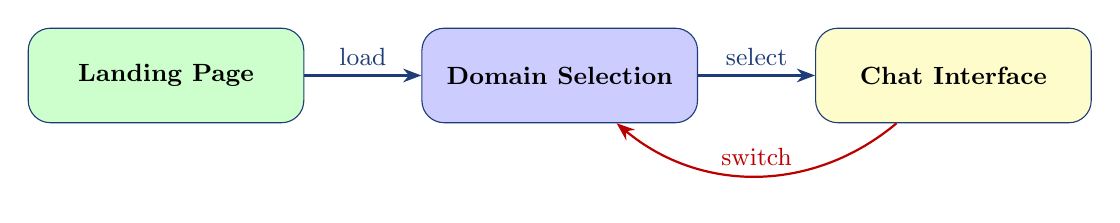
\begin{tikzpicture}[node distance=2.5cm]
        % States
        \node[component, fill=green!20, minimum width=3.5cm] (start) at (0, 0) {Landing Page};
        \node[component, fill=blue!20, minimum width=3.5cm] (select) at (5, 0) {Domain Selection};
        \node[component, fill=yellow!20, minimum width=3.5cm] (chat) at (10, 0) {Chat Interface};
        
        % Arrows
        \draw[arrow] (start) -- node[above]{\small load} (select);
        \draw[arrow] (select) -- node[above]{\small select} (chat);
        \draw[arrow, color=univrred] (chat) to[bend left=40] node[above]{\small switch} (select);
    \end{tikzpicture}
    \caption{Frontend navigation flow}
    \label{fig:frontend-flow}
\end{figure}

\subsection{Domain Selection Screen}

When the user first opens the application:

\begin{enumerate}
    \item The frontend fetches available domains from the backend (\texttt{GET /api/domains})
    \item Domains are displayed as clickable cards with:
    \begin{itemize}
        \item Domain name (e.g., ``Scholarships'')
        \item Document count (e.g., ``5 documents'')
    \end{itemize}
    \item User clicks a domain to enter the chat interface
\end{enumerate}

\subsection{Chat Interface}

Once a domain is selected, the user enters the chat interface:

\begin{figure}[H]
    \centering
    \begin{tikzpicture}[node distance=0.8cm]
        % Container
        \draw[rounded corners=10pt, fill=univrbg] (-4, -5) rectangle (4, 4);
        
        % Header
        \draw[fill=white, rounded corners=5pt] (-3.8, 3.2) rectangle (3.8, 3.8);
        \node at (0, 3.5) {\small\bfseries Scholarships | UniVR Chatbot};
        
        % Messages area
        \draw[fill=white!80, rounded corners=5pt] (-3.8, -2) rectangle (3.8, 3);
        
        % Bot message
        \draw[fill=lightblue, rounded corners=5pt] (-3.5, 2) rectangle (1.5, 2.7);
        \node at (-1, 2.35) {\tiny Welcome! Ask me anything...};
        
        % Suggestions
        \draw[fill=green!15, rounded corners=3pt] (-3.5, 0.8) rectangle (1, 1.3);
        \node at (-1.25, 1.05) {\tiny 💡 What scholarships are available?};
        \draw[fill=green!15, rounded corners=3pt] (-3.5, 0.2) rectangle (1.2, 0.7);
        \node at (-1.15, 0.45) {\tiny 💡 What are the deadlines?};
        
        % User message
        \draw[fill=univrred!25, rounded corners=5pt] (-0.5, -0.8) rectangle (3.5, -0.1);
        \node at (1.5, -0.45) {\tiny How do I apply for a scholarship?};
        
        % Bot response
        \draw[fill=lightblue, rounded corners=5pt] (-3.5, -1.8) rectangle (2, -1.1);
        \node at (-0.75, -1.45) {\tiny To apply, you need to submit...};
        
        % Input area
        \draw[fill=white, rounded corners=5pt] (-3.8, -4.8) rectangle (3.8, -2.3);
        \draw[fill=gray!10, rounded corners=3pt] (-3.5, -4.5) rectangle (2.8, -3.8);
        \node[anchor=west] at (-3.3, -4.15) {\tiny Ask about scholarships...};
        \draw[fill=univrred, rounded corners=3pt] (3, -4.5) rectangle (3.6, -3.8);
        \node at (3.3, -4.15) {\tiny\color{white} →};
        
        % Footer
        \node at (0, -3) {\tiny Powered by Gemini AI with RAG};
    \end{tikzpicture}
    \caption{Chat interface mockup showing key UI elements}
    \label{fig:chat-mockup}
\end{figure}

\subsection{Key UI Components}

\begin{table}[H]
    \centering
    \begin{tabular}{@{}lp{9cm}@{}}
        \toprule
        \textbf{Component} & \textbf{Description} \\
        \midrule
        Header & Shows current domain, dark mode toggle, domain switch button \\
        Welcome Message & Greets user and introduces the chatbot's capabilities \\
        Suggested Questions & AI-generated questions based on domain documents \\
        Message History & Scrollable list of user/bot messages with formatting \\
        Source Citations & References to documents used in responses \\
        Input Area & Text input with send button, supports Enter key \\
        Loading Indicator & Animated dots while waiting for response \\
        \bottomrule
    \end{tabular}
    \caption{Frontend UI components}
\end{table}

\subsection{Interaction Flow}

\begin{figure}[H]
    \centering
    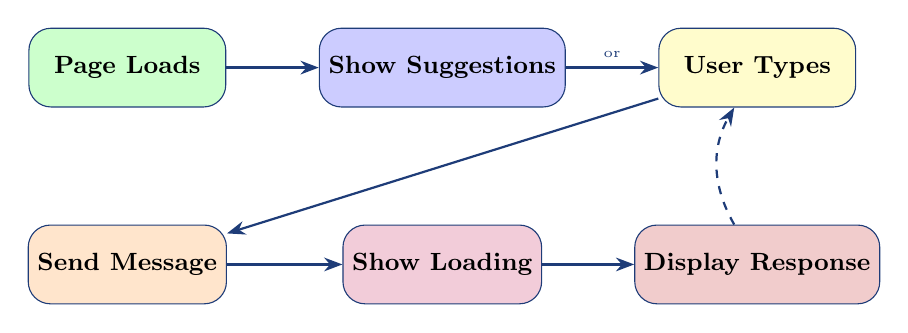
\begin{tikzpicture}[node distance=1.8cm]
        % Actions
        \node[component, fill=green!20, minimum width=2.5cm, minimum height=1cm] (load) at (0, 0) {Page Loads};
        \node[component, fill=blue!20, minimum width=2.5cm, minimum height=1cm] (suggest) at (4, 0) {Show Suggestions};
        \node[component, fill=yellow!20, minimum width=2.5cm, minimum height=1cm] (input) at (8, 0) {User Types};
        \node[component, fill=orange!20, minimum width=2.5cm, minimum height=1cm] (send) at (0, -2.5) {Send Message};
        \node[component, fill=purple!20, minimum width=2.5cm, minimum height=1cm] (loading) at (4, -2.5) {Show Loading};
        \node[component, fill=univrred!20, minimum width=2.5cm, minimum height=1cm] (display) at (8, -2.5) {Display Response};
        
        % Arrows
        \draw[arrow] (load) -- (suggest);
        \draw[arrow] (suggest) -- node[above]{\tiny or} (input);
        \draw[arrow] (input) -- (send);
        \draw[arrow] (send) -- (loading);
        \draw[arrow] (loading) -- (display);
        \draw[arrow, dashed] (display) to[bend left=30] (input);
    \end{tikzpicture}
    \caption{User interaction flow within the chat interface}
    \label{fig:interaction}
\end{figure}

%==============================================================================
% Section 6: Domain Management
%==============================================================================
\section{Domain Management}

\subsection{Domain Concept}

A \textbf{domain} in the UniVR Chatbot represents a specific area of knowledge, such as:
\begin{itemize}
    \item \textbf{Scholarships}: ESU grants, merit awards, international student funding
    \item \textbf{Admissions}: Application procedures, requirements, deadlines
    \item \textbf{Tuition}: Fee structures, payment schedules, exemptions
    \item \textbf{International}: Visa procedures, exchange programs, support services
\end{itemize}

\subsection{Domain Creation Workflow}

\begin{figure}[H]
    \centering
    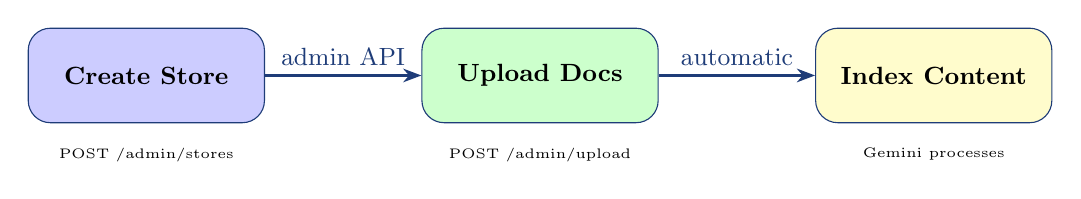
\begin{tikzpicture}[node distance=2cm]
        % Steps
        \node[component, fill=blue!20] (create) at (0, 0) {Create Store};
        \node[component, fill=green!20] (upload) at (5, 0) {Upload Docs};
        \node[component, fill=yellow!20] (index) at (10, 0) {Index Content};
        
        % Arrows
        \draw[arrow] (create) -- node[above]{\small admin API} (upload);
        \draw[arrow] (upload) -- node[above]{\small automatic} (index);
        
        % Labels below
        \node[anchor=north, font=\tiny] at (0, -0.8) {POST /admin/stores};
        \node[anchor=north, font=\tiny] at (5, -0.8) {POST /admin/upload};
        \node[anchor=north, font=\tiny] at (10, -0.8) {Gemini processes};
    \end{tikzpicture}
    \caption{Domain creation and document indexing process}
    \label{fig:domain-creation}
\end{figure}

\subsection{Document Processing}

When a document is uploaded to a domain:

\begin{enumerate}
    \item \textbf{Upload}: File is sent to Gemini's File API
    \item \textbf{Metadata Extraction}: AI extracts title and abstract
    \item \textbf{Duplicate Check}: Existing file with same name is replaced
    \item \textbf{Indexing}: Content is vectorized and added to the File Search Store
    \item \textbf{Availability}: Document becomes searchable for RAG queries
\end{enumerate}

%==============================================================================
% Section 7: Suggested Questions Feature
%==============================================================================
\section{AI-Generated Suggestions}

\subsection{How Suggestions Work}

One unique feature of the UniVR Chatbot is the ability to generate \textbf{context-aware suggested questions} based on the documents in each domain.

\begin{figure}[H]
    \centering
    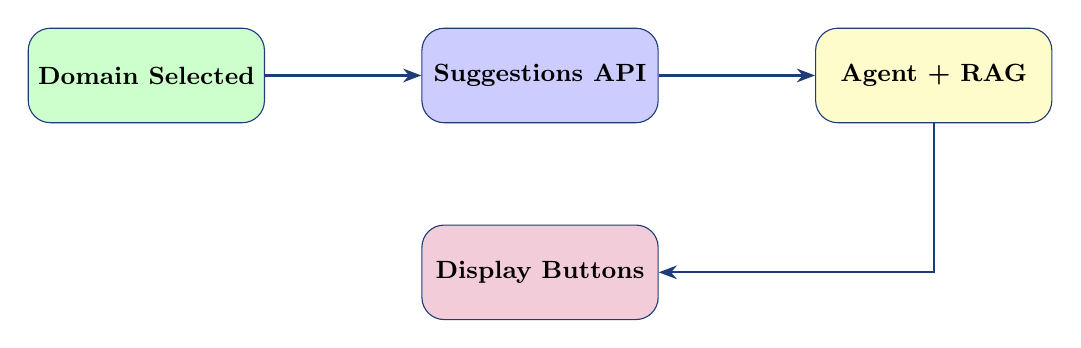
\begin{tikzpicture}[node distance=1.5cm]
        % Process
        \node[component, fill=green!20] (domain) at (0, 0) {Domain Selected};
        \node[component, fill=blue!20] (api) at (5, 0) {Suggestions API};
        \node[component, fill=yellow!20] (agent) at (10, 0) {Agent + RAG};
        \node[component, fill=purple!20] (display) at (5, -2.5) {Display Buttons};
        
        % Arrows
        \draw[arrow] (domain) -- (api);
        \draw[arrow] (api) -- (agent);
        \draw[arrow] (agent) |- (display);
    \end{tikzpicture}
    \caption{Suggestion generation workflow}
    \label{fig:suggestions}
\end{figure}

\subsection{Benefits}

\begin{itemize}
    \item \textbf{Discoverability}: Users learn what information is available
    \item \textbf{Quick Start}: One-click to start a relevant conversation
    \item \textbf{Dynamic Content}: Questions update based on actual documents
    \item \textbf{Reduced Friction}: No need to formulate complex queries
\end{itemize}

%==============================================================================
% Section 8: Use Cases
%==============================================================================
\section{Use Cases}

\subsection{Student Scenarios}

\begin{tcolorbox}[colback=green!5, colframe=green!60!black, title=\textbf{Scholarship Application}]
    \textbf{Scenario}: A student wants to know about ESU scholarships.
    
    \textbf{Flow}:
    \begin{enumerate}[noitemsep]
        \item Student selects ``Scholarships'' domain
        \item Sees suggested question: ``What are the ESU scholarship requirements?''
        \item Clicks the suggestion or asks a custom question
        \item Receives detailed answer with deadlines and links
    \end{enumerate}
\end{tcolorbox}

\vspace{0.5cm}

\begin{tcolorbox}[colback=blue!5, colframe=blue!60!black, title=\textbf{International Student}]
    \textbf{Scenario}: An international student needs visa information.
    
    \textbf{Flow}:
    \begin{enumerate}[noitemsep]
        \item Student selects ``International'' domain
        \item Asks: ``What documents do I need for a study visa?''
        \item Chatbot retrieves relevant policies and lists requirements
        \item Sources are cited for official verification
    \end{enumerate}
\end{tcolorbox}

%==============================================================================
% Section 9: Conclusion
%==============================================================================
\section{Conclusion}

\subsection{Summary}

The UniVR Chatbot provides a modern, AI-powered solution for student information access. By combining:
\begin{itemize}
    \item \textbf{RAG Technology} for accurate, document-grounded responses
    \item \textbf{Multi-Domain Architecture} for organized knowledge management
    \item \textbf{Intuitive Frontend} for seamless user experience
    \item \textbf{AI-Generated Suggestions} for content discovery
\end{itemize}

\subsection{Future Enhancements}

Potential improvements include:
\begin{itemize}
    \item Conversation history persistence
    \item User authentication for personalized responses
    \item Analytics dashboard for admin insights
    \item Multi-modal support (images, forms)
    \item Voice input/output capabilities
\end{itemize}

%==============================================================================
% End Document
%==============================================================================
\end{document}
